\renewcommand{\thefigure}{Fig.~\arabic{figure}}
\renewcommand{\thetable}{Table~\arabic{table}}

%%% TITLE %%%
\title{\Large \bf Canalization of the evolutionary trajectory of the human influenza virus}
\maketitle

\begin{abstract}
\noindent \bf Influenza A (H3N2) has persisted in the human population since 1968 through continued seasonal epidemics.  During this time, the influenza virus underwent substantial antigenic drift, allowing it to infect a large fraction of the human population year after year.  Understanding the process of antigenic evolution is key to our efforts of disease control and surveillance; the continual emergence of new antigenic variants requires corresponding updates to the influenza vaccine.  The antigenic evolution of H3N2 influenza has been experimentally characterized, resulting in an two-dimensional `antigenic map' describing antigenic similarity and distance between strains \cite{Smith04}.  The genetic relationships among H3N2 strains have also been distinguished, showing a characteristic ladder-like genealogical tree \cite{Fitch97}.  This work seeks to simultaneously model epidemiological, antigenic, genealogical and spatial patterns of the influenza virus.  Here, we use a large-scale individual-based model to show that evolution in a Euclidean antigenic space results a remarkable correspondence between model behavior and available data.  We find that evolution away from human immunity results in rapid population turnover in the influenza virus and that this population turnover occurs primarily along a single antigenic axis.  Thus, selective dynamics induce a canalized evolutionary trajectory, in which the evolutionary fate of the influenza population is surprisingly repeatable and hence, in theory, predictable.
\end{abstract}

Epidemic influenza is responsible for between 250,000 and 500,000 global deaths annually, with influenza A (H3N2) having historically caused the bulk of human mortality and morbidity \cite{flufactsheet}.  Since its emergence, influenza A H3N2 has continually evolved both genetically and antigenically.  Most antigenic drift is thought to be driven by changes to epitopes in the hemagglutinin (HA) protein \cite{Nelson07NatRevGenet}.  Phylogenetic analysis of the genetic relationships among HA sequences has revealed a distinctive genealogical tree showing a single predominant trunk lineage and side branches that persist for only 1--5 years before going extinct \cite{Fitch97}.  This tree shape is indicative of serial replacement of strains over time; H3N2 influenza shows rapid evolution, but low standing genetic diversity.

This observation has remained puzzling from an epidemiological standpoint.  Antigenic evolution occurs rapidly and strong diversifying selection exists to escape from human immunity; why then do we see serial replacement of strains rather than continual genetic and antigenic diversification?  Indeed, simple epidemiological models show explosive diversity of genotype and phenotype over time \cite{Ferguson03,Tria05}.  Previous work has sought model-based explanations of the limited diversity of influenza, relying on short-lived strain-transcending immunity \cite{Ferguson03,Tria05}, complex genotype-to-phenotype maps \cite{Koelle06} or a limited repertoire of antigenic phenotypes \cite{Recker07}. 

Experimental characterization of antigenic phenotype is possible through the hemagglutination inhibition (HI) assay, which measures the cross-reactivity of HA from one virus strain to serum raised against another strain \cite{Hirst43}.  The results of many HI assays can be combined to yield a two-dimensional map, representing antigenic similarity and distance between strains as an easily visualized and quantified measure \cite{Smith04}.  The path traced across this map by influenza A (H3N2) from 1968 until present is largely linear, showing serial replacement of one strain by another; there are no major bifurcations of antigenic phenotype \cite{Smith04}.

Herein, we seek to reconcile antigenic and genetic patterns of influenza evolution using a large-scale individual-based model.  Our model begins with the finding of Smith et al.\ \cite{Smith04}, that a two-dimensional map adequately explains observed antigenic distance between strains.  Here, in an analogous fashion, we represent antigenic phenotypes as points on a plane.  After exposure to a virus, a host's risk of infection is proportional to the Euclidean distance between the infecting phenotype and the closest phenotype in the host's immune history.  Mutations perturb antigenic phenotype, moving phenotype in a random radial direction and for a randomly distributed distance.  

We implemented this geometrical model in a large-scale individual-based simulation intended to simultaneously and directly model the antigenic map and genealogical tree of the global influenza population (for details see Methods).  The simulation includes multiple host populations with different seasonal forcings, hosts with complete immune histories of infection, and viruses with antigenic phenotypes.  As the simulation proceeds, infections are tracked and a complete genealogy connecting virus samples is constructed.  This avoids the messy intermediate step of phylogenetic inference common to phylodynamic simulations, and allows large genealogies to be reconstructed quickly and without error.  Results shown here are for a single simulation of 40 years of virus evolution in a population of 90 million hosts.  

The virus persists over the course of the 40-year simulation, infecting a significant fraction of the host population through annual winter epidemics in temperate regions and through less periodic epidemics in the tropics (\ref{incmaptree}A).  Across replicate simulations, we observe average yearly attack rates of 6.8\% in temperate regions and rates of 7.1\% in the tropics, matching attack rates of influenza A (H3N2) estimated at 3--8\% per year \cite{Monto93,Koelle09}.  Over the course of the simulation, the virus population evolves in antigenic phenotype (\ref{incmaptree}B, \ref{phenotypes}A).  The appearance of clusters in the antigenic map (\ref{incmaptree}B) comes from the regular spacing of high abundance phenotypes (\ref{phenotypes}A) combined with measurement noise (see Methods).  Over the course of the simulation, clusters of antigenically similar strains are replaced by novel clusters of more advanced strains (\ref{incmaptree}B, \ref{phenotypes}B).  

Remarkably, although antigenic phenotype is free to mutate in any direction in the two-dimensional space, selection pressures force the virus population to move in nearly a straight line in antigenic space (\ref{incmaptree}B, \ref{phenotypes}A).  Across replicate simulations, 94\% of the variance of antigenic phenotype can be explained by a single dimension of variation.  This mirrors the empirical results showing a largely linear antigenic map for H3N2 influenza isolates from 1968 to 2003 \cite{Smith04}.  Because of the primarily one-dimensional movement, antigenic distance from the original phenotype increases linearly with time (\ref{phenotypes}C).  Antigenic evolution occurs in a punctuated fashion; periods of relative stasis are interspersed with more rapid antigenic change resulting in a fundamental linkage of evolutionary and epidemiological dynamics (see Supp.~Discussion).

The genealogical tree connecting the evolving virus population appears characteristically sparse with pronounced trunk and short-lived side branches  (\ref{incmaptree}C).  This tree shape is reflected in low levels of standing diversity; across replicates, an average of 5.68 years of evolution separate two randomly sampled viruses in the population.  This level of diversity matches what is observed in phylogenies of influenza A (H3N2) \cite{Rambaut08}.  A spindly genealogical tree is indicative of population turnover, wherein novel antigenic phenotypes continually replace more primitive `spent' phenotypes, purging their genealogical diversity.  In general, natural selection reduces effective population size and genealogical diversity \cite{BedfordBMC11}.  Here, by comparing mutations occuring on trunk branches vs.\ mutations occurring on side branches, we find evidence for pervasive positive selection for antigenic change (\ref{mktable}).  Trunk mutations tend to push antigenic phenotype forward along the line of primary antigenic variation (\ref{mutspectrum}, \ref{probtrunk}).  Additionally, we find that trunk mutations occurred at unexpectedly regular intervals, with less variation of waiting times than expected under a simple random process (\ref{waittimes}).

The genealogical tree also contains detailed information on the history of migration between regions.  We find that, consistent with empirical estimates \cite{Russell08,Bedford10}, the trunk resides primarily within the tropics, where seasonal dynamics are less prevalent (\ref{spatial}A).  Across replicate simulations, we observe 72\% of the trunk's history within the tropics and 28\% within temperate regions.  With symmetric host contact rates and equivalent host population sizes, and without seasonal forcing, we would expect trunk proportions of one third for each region.  We calculated rates of migration based on observed event counts across replicate simulations, separating region-specific rates on side branches (\ref{spatial}B) from region-specific rates on trunk branches (\ref{spatial}C).  We find that migration patterns on side branches are close to symmetric, with similar rates between all regions (\ref{spatial}B).  However, migration patterns on trunk branches are highly asymmetric, with high rates of movement between temperate regions and from temperate regions into the tropics (\ref{spatial}C).  Extrapolating from these rates, we arrive at an expected stationary distribution of 76\% tropics and 24\% temperate regions, in line with the observed residency patterns of the trunk.  These findings suggest that persistence and migration are fundamentally connected and have important implications for future phylogeographic analyses (see Supp.\ Discussion).

Although multiple epidemiological/evolutionary mechanisms have been proposed to explain the restricted genetic diversity and rapid population turnover of influenza A (H3N2) \cite{Ferguson03,Tria05,Koelle06,Recker07}, our results show that a simple model coupling antigenic and genealogical evolution exhibits remarkable explanatory power.  We find a strong correspondence between the antigenic and genealogical patterns generated by our model (\ref{incmaptree}B--C) and patterns of genetic and antigenic evolution exhibited by influenza A (H3N2) \cite{Fitch97,Smith04}.  This underlies the importance of further characterizing antigenic space, especially in relation to epitope structure \cite{Recker07}, and suggests that antigenic evolution is primarily limited by a lack of mutational input and not by short-lived transcending immunity (see Supp.~Discussion).  Additionally, our model can be extended to describe the dynamics of other types/subtypes of influenza by simply lowering mutational input or lowering intrinsic $R_0$.  By doing so, our model exhibits decreased incidence, slower antigenic movement and greater genealogical diversity, all distinguishing characteristics of H1N1 influenza and influenza B (\ref{h1n1_mut}, \ref{h1n1_r0}).

It would seem possible for one viral lineage to move in one antigenic direction, while another lineage moves tangentially, eventually resulting in two non-interacting viral lineages.  Instead, we find that only movement in a single antigenic direction is favored.  The origins of this pattern can be seen in the interaction between virus evolution and host immunity (\ref{immunity}).  As the virus population evolves forward it leaves a wake of immunity in the host population, and evolution away from this immunity results in the canalization of the antigenic phenotype; mutations that continue along the line of primary antigenic variation will show a transmission advantage compared to more tangential mutations.  

Following the work of Smith et al.\ \cite{Smith04}, it remained an open question of why a two-dimensional map should explain the antigenic variation of H3N2 influenza.  Although the authors astutely speculated that ``there is a selective advantage for clusters that move away linearly from previous clusters as they most effectively escape existing population-level immunity, and this is a plausible explanation for the somewhat linear antigenic evolution in regions of the antigenic map.''  This hypothesis remained to be tested.  Here, we show from a simple model of epidemiology and evolution that a linear trajectory of antigenic evolution dynamically emerges due basic selective pressures.  This result simultaneously explains the linear pattern of antigenic drift \cite{Smith04} and the characteristically spindly genealogical tree \cite{Fitch97} exhibited by influenza A (H3N2).

Still, we were uncertain to what extent these results were contingent on the dimensionality of the underlying antigenic model.  We tested this by implementing our model in a 10-dimensional antigenic space.  Here, mutations occur as 10-spheres, but the distance moved by a mutation is the same as in the previous two-dimensional formulation.  We arrive at nearly the same results with this model; principal components analysis shows that the first and second dimensions of variation account for 87\% and 7\%, respectively, of the total variance (\ref{10dgrid}).  Thus, even if the underlying antigenic space of H3N2 influenza were high dimensional, we could find a two-dimensional map sufficient to explain observed antigenic relationships among strains.

It seems clear that, in our model, selection reduces the degrees of freedom of antigenic evolution.  In light of this, we wanted to examine the degree of stochasticity in replicated evolutionary trajectories, and thereby test what happens when we ``wind back the tape'' \cite{GouldWonderfulLife} on the evolution of the virus.  We ran 100 replicate simulations, each starting from the endpoint of the original 40-year simulation (\ref{replicateevol}).  Initially, we find a great detail of repeatability.  During the first year of evolution, every replicate virus population undergoes a similar antigenic transition (\ref{replicateevol}).  As time continues there is growing dissimilarity between replicates, and at the end of 4 years, replicate populations differ substantially (\ref{replicateevol}).  The 1--2 year timescale of repeatability can be explained by the presence of standing antigenic variation.  In the initial virus population, there are several novel antigenic variants present at low frequency (\ref{replicateevolfull}).  Without fail, one of these novel antigenic variants comes to predominate, resulting in a repeatable peak in northern hemisphere incidence (\ref{replicatetimeseries}).  After three years, repeatability has mostly disappeared, with antigenic phenotype and incidence appearing highly variable across replicates (\ref{replicateevol}, \ref{replicatetimeseries}).

We see that the initial evolutionary trajectory, during which time standing variation plays out, is highly repeatable, and thus predictable given enough information and the right methods of analysis.  However, prediction of longer-term evolutionary scenarios will necessarily be difficult or impossible except in a vague sense.  Through careful surveillance efforts and genetic and antigenic characterization of influenza strains, the World Health Organization makes twice-yearly vaccine strain recommendations \cite{Barr10}.  It may be possible to combine these sorts of modeling approaches with surveillance data to gauge the likelihood that a sampled variant will spread through the population.

Recent work on empirical fitness landscapes has shown that natural selection follows few mutational paths \cite{Weinreich06}.  The spindly genealogical tree and serial replacement of influenza strains has remained a puzzling phenomenon.  We suggest that the evolutionary and epidemiological dynamics displayed by the influenza virus may be explained as an outgrowth of selection to avoid host immunity.  Natural selection can only `see' one step ahead, and so sacrifices long-term gains for short-term success.  The result is a canalized evolutionary trajectory lacking antigenic diversification.

\subsection*{Methods summary}

To characterize the joint epidemiological, genealogical, antigenic and spatial patterns of influenza, we implemented a large-scale individual-based model.  This model consists of daily time steps, in which the states of hosts and viruses are updated.  Hosts may be born, may die, may contact other hosts allowing viral transmission, or may recover from infection.  Viruses may mutate in antigenic phenotype.

Our model follows Gog and Grenfell \cite{Gog02} in representing antigenic distance as distance between points on a geometric space.  By forcing one-dimension to directly modulate $\beta$, Gog and Grenfell find an orderly replacement of strains.  Kryazhimskiy et al. \cite{Kryazhimskiy07} use a two-dimensional strain-space, but enforce a cross-immunity kernel that directly favors moving along a diagonal line away from previous strains.  Our model does not `build in' the one-dimensional direction of antigenic drift, which instead emerges dynamically from competition among strains.

% We implemented our epidemiological and evolutionary model in a large-scale individual-based simulation describing 40 years of virus evolution in a population of 90 million host individuals.  Hosts were divided into three regional populations: North, South and Tropics.  Temperate populations undergo seasonal forcing with opposite phases, while ehe tropics population has no seasonal forcing.  Each day, hosts make contacts with one another allowing infection to spread, and recover from infection generating full immunity to the specific infecting phenotype. With each exposure event, the risk of infection is determined from comparing the phenotype of the infecting virus to all the phenotypes in the host's immune history.  Over time, viruses mutate in antigenic phenotype.  As the simulation proceeds, we record daily incidence and we sample infections and record phenotype, location and ancestry of each sampled virus.

%%% REFERENCES %%%
\bibliographystyle{plos2009}
\bibliography{/Users/bedfordt/Documents/bedford}

\pagebreak

%%% FIGURES %%%
\section*{Figures}

%%% Figure 1: incmaptree %%%
\begin{figure}[H]
	\centering
	\includegraphics{figures/incmaptree}
	\caption{\textbf{Simulation results showing epidemiological, antigenic and genealogical dynamics}. (A) Weekly timeseries of incidence of viral infection in north and tropics regions. (B) Antigenic map depicting phenotypes of 5943 viruses sampled over the course of the simulation.  To construct the map, noise was added to each sample and the resulting observations grouped into 10 clusters and colored accordingly.  Grid lines show single units of antigenic distance. (C) Genealogical tree depicting the infection history of 376 samples from the virus population.  Parent/offspring relationships were tracked over the course of the simulation, giving a direct observation of the genealogy rather than a phylogenetic inference. Cluster assignments were used to color panels (A), (B) and (C) in a consistent fashion.}
	\label{incmaptree}
\end{figure}

\pagebreak

%%% Figure 2: spatial %%%
\begin{figure}[H]
	\centering
	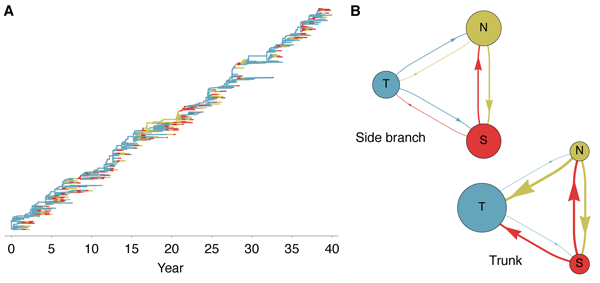
\includegraphics{figures/spatial}
	\caption{\textbf{Patterns of spatial movement of virus lineages}. (A) Evolutionary relationships among 367 viruses sampled evenly through time colored by spatial location. Lineages residing in the north (N), south (S) and tropics (T) are colored yellow, red and blue respectively. (B) Migration rates between regions on side branch lineages, and (C) Migration rates between regions on trunk lineages. Arrows denote movement of lineages and arrow width is proportional to migration rate. Circle area is proportional to the expected stationary frequency of a region given the observed migration rates.  In both cases, migration rates are calculated across 80 replicate simulations.}
	\label{spatial}
\end{figure}

%%% Figure 3: immunity %%%
\begin{figure}[H]
	\centering
	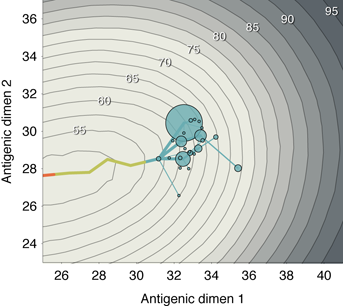
\includegraphics{figures/immunity}
	\caption{\textbf{Host immunity and antigenic history of the virus population}.  Contour lines represent the state of host immunity at the end of the 40-year simulation.  They show the mean risk of infection (as a percentage) after a random host in the population encounters a virus bearing a particular antigenic phenotype.  Contour lines are spaced in intervals of 2.5\%. Bubbles represent a sample of antigenic phenotypes present at the end of the 40-year simulation.  The area of each bubble is proportional to the number of samples with this phenotype.  Lines leading into these bubbles show past antigenic history.  The current phenotypes rapidly coalesce to a trunk phenotype.  The movement of the virus population from top left to the center of the figure can be seen from the antigenic history of the trunk of the virus genealogy. At the end of the simulation several virus phenotypes exist with similar antigenic locations; all of these phenotypes lie significantly ahead of the peak of host immunity.}
	\label{immunity}
\end{figure}

%%% Figure 4: replicateevol %%%
\begin{figure}[H]
	\centering
	\makebox[\textwidth]{	
		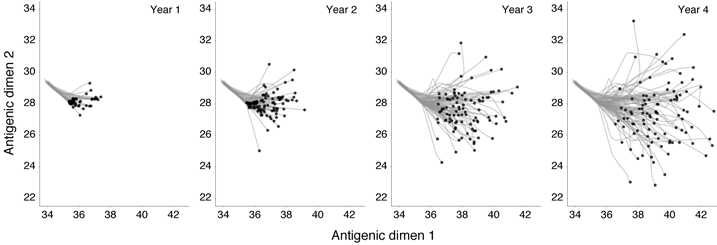
\includegraphics{figures/replicateevol}
	}
	\caption{\textbf{Antigenic phenotypes over the course of 5 years of evolution across 100 replicate simulations starting from identical initial conditions}.  Replicate simulations were initialized with the end state of the original 40-year simulation shown in \ref{incmaptree}.  Each panel shows an additional year of evolution, with black points representing the mean antigenic phenotypes of the 100 replicate simulations and gray lines representing the history of each mean antigenic phenotype.}
	\label{replicateevol}
\end{figure}
